\documentclass[12pt]{exam}  % exam document class - MIT Mathematics
\usepackage[utf8]{inputenc}

\usepackage{tikz}
\usepackage{pgfplots}

\usetikzlibrary{math}
%\usetikzlibrary{datavisualization.formats.functions}
%\usetikzlibrary{datavisualization}
\usetikzlibrary{intersections}
\pgfplotsset{compat=1.16}


\usepackage{xcolor}
\usepackage{colortbl}
\usepackage{amsmath}
\usepackage{amssymb}
\usepackage{gnuplottex}
\usepackage{graphicx}
\usepackage{siunitx}
\usepackage{multicol}
\usepackage{tasks}
\usepackage{physics}
\usepackage{cancel}
\usepackage{todonotes}
\usepackage{romannum}

\renewcommand{\solutiontitle}{\noindent\textbf{Lösung:}\par\noindent}

\renewcommand{\questionshook}{%
\setlength{\leftmargin}{0pt}%
\setlength{\labelwidth}{-\labelsep}%
}

\newcommand{\uuline}[1]{\underline{\underline{~#1~}}}

\setlength{\jot}{8pt}

\settasks{
    label-width = 11.0971pt
  }


%%%%%%%%% Ausgabe der Lösungen %%%%%%%%%

%\noprintanswers
\printanswers

%%%%%%%%% Rahmen um Lösung %%%%%%%%%
\unframedsolutions
%\framedsolutions

\begin{document}
		\pagestyle{headandfoot}

\firstpageheader{Übungsaufgaben\\ Bodendynamik}{TU Bergakademie Freiberg \\Institut für Geotechnik}{Seite \thepage\ von \numpages\\}
\firstpageheadrule

\firstpagefooter{}{}{}
\runningfooter{}{}{}

\runningheader{Übungsaufgaben\\ Bodendynamik}{TU Bergakademie Freiberg \\Institut für Geotechnik}{Seite \thepage\ von \numpages\\}
\runningheadrule
\runningfootrule

\setlength{\jot}{8pt}


%%% Todonotes margin - remove when done
\setlength {\marginparwidth }{2cm}
		\tikzset{
%DKspring(length) length=2...10
DKspring/.pic={
\coordinate (half_up) at (0.5*0.125*#1-0.5*0.125*2, 0.5*0.125*10-0.5*0.125*#1); %at (0.5*(#1-0.2), 0.5*(1.0-#1));
\coordinate (full_up)   at ( 0.125*#1-    0.125*2,     0.125*10-    0.125*#1);
\coordinate (full_down) at ( 0.125*#1-    0.125*2,    -0.125*10+    0.125*#1);
\draw (0, 0) -- ++(1, 0) -- ++(half_up)
    -- ++(full_down) -- ++(full_up) 
    -- ++(full_down) -- ++(full_up)
    -- ++(full_down) -- ++(full_up)
    -- ++(full_down) -- ++(half_up)
    -- ++(1, 0);
    },   
%DKdashpot(length) length=02...10    
DKdashpot/.pic={
\coordinate (upper_end) at (#1-0.5, 0.5);
\coordinate (lower_end) at (#1-0.5,-0.5);
\coordinate (upper_pos) at (#1-1, 0.5);
\coordinate (lower_pos) at (#1-1,-0.5);
\coordinate (center_pos) at (#1-1, 0.0);
\coordinate (center_end) at (#1, 0.0);
\draw (0, 0) -- ++(1, 0);
\draw (upper_end) -- (1, 0.5) -- (1, -0.5) -- (lower_end);
\draw (center_pos) -- (center_end);
\draw (upper_pos) -- (lower_pos);
    },
DKbase/.pic={
\draw[thick] (0, 1.5) -- (0, -1.5);
\foreach \y in {-1.5,-1.0,...,1.0} \draw[thin] (0, \y) -- +(-0.5, 0.5);
},
 invisible/.style={opacity=0},
  visible on/.style={alt={#1{}{invisible}}},
  alt/.code args={<#1>#2#3}{%
    \alt<#1>{\pgfkeysalso{#2}}{\pgfkeysalso{#3}} % \pgfkeysalso doesn't change the path
  }
}

	\begin{coverpages}
		\huge\centering Übungsaufgaben Bodendynamik - SS \the\year 
		\normalsize
	\end{coverpages}
	
	\begin{questions}
	
		\section{Einleitung}
		%\fullwidth{\Large \textbf{Essay questions}}
		\question{Recherche}   
Suchen Sie nach Nachrichten mit Geotechnikbezug.

\begin{solution}
Der Weg ist das Ziel 
\end{solution}

%%%%%%%%%%%%%%%%%%%%%%%%%%%%%%%%%%%%%%%%%%%%%%%%%%%%%%%%%%%%%%%%%%%%%%%%%%%%%%

\question{Online--Ressourcen}
Suchen Sie nach Videos und interaktivem Material zu geotechnischen Schlagwörtern.

\begin{solution}
Der Weg ist das Ziel 
\end{solution}

%%%%%%%%%%%%%%%%%%%%%%%%%%%%%%%%%%%%%%%%%%%%%%%%%%%%%%%%%%%%%%%%%%%%%%%%%%%%%

\question{Woher können im Verkehrsnetz Erschütterungen kommen? Warum ist ggf. ein Erschütterungsschutz für umstehende Gebäude notwendig?}

\begin{solution}
    Der Weg ist das Ziel 
\end{solution}

%%%%%%%%%%%%%%%%%%%%%%%%%%%%%%%%%%%%%%%%%%%%%%%%%%%%%%%%%%%%%%%%%%%%%%%%%%%%

\question{Informieren Sie sich über die Funktionsweise eines Erdbebenfrühwarnsystems.}

		
		\newpage
		\section{Grundlagen}
		   \subsection{Einfreiheitsgradschwingungen}
		   \question{Erzwungene, ungedämpfte Schwingung}
\vspace{1em}

     \begin{tikzpicture}[scale=0.6]
 \fill[black!5!white] (-1,-2) rectangle (7, 3); 
\draw[->] (2.5, 2) --(4, 2);
\draw (2.5,1.8) -- (2.5, 2.2);
\draw[thin] (4,1.5)--(4,2.2);
\draw (0, 0) pic [scale=0.6] {DKbase};
\draw (0, 0) pic [scale=0.6, thick] {DKspring=4};  
\draw[thick] (4,-1.5) rectangle +(1.5, 3); 
\draw (2, -0.9) node {$k$};
\draw (4.7, 0) node {$m$};
\draw (3.25, 2.3) node {$u$};
\draw[->, very thick] (5.7, 0) -- (6.9, 0);
\draw (6.25, 0.55) node {$F(t)$};
\end{tikzpicture}


    \begin{minipage}[t]{.49\linewidth}
    geg.:
    \begin{tasks}(2)
        \task[] $m = \SI{3}{\kilo\gram}$
        \task[] $k = \SI{10}{\newton\per\meter}$
        \task[] $F(t) = \hat{F} \sin{\omega t}$
        \task[] $\hat{F} = \SI{5}{\newton}$
        \task[] $\omega = \SI{10}{\radian\per\second}$
        \task[] $t=\SI{0}{\second}$
        \task[] $u_0 = \SI{0.1}{m}$
        \task[] $\dot{u}_0 = \SI{0}{\meter\per\second}$
    \end{tasks}
    \end{minipage}
    \begin{minipage}[t]{.49\linewidth}
    ges.:
    \begin{tasks}
        \task $u(t)$
    \end{tasks}
    \end{minipage}

    \begin{solution}
        \begin{alignat*}{2}
            &(c = \SI{0}{\newton\second\per\meter}, F_C = \SI{0}{\newton}, F_S = \hat{F} = \SI{5}{\newton})\\
            &\omega_0 = \sqrt{k/m} &&= \SI{1.826}{\radian\per\second} \\
            &\zeta = \frac{c}{2\sqrt{mk}} &&= 0 \\
            &\eta = \omega/\omega_0 &&= 5.477\\
            &V = (1-\eta^2)^{-1} &&=  0.0345 \\
            &u_C = -2V^2\zeta\eta\hat{F}/k &&= \SI{0}{\meter} \\
            &u_S = V^2(1-\eta^2)\hat{F}/k &&= \SI{-0.0172}{\meter}
        \end{alignat*}

        \begin{align*}
            u_0 &= C_1 + u_C \\
            \dot{u}_0 &= \omega_0 C_2+\omega u_S\\
            &\rightsquigarrow \\
            C_1 &=  u_0 - U_C = \SI{0.1}{\meter}\\
            C_2 &= \frac{\dot{u}_0 - \omega u_S}{\omega_0} = \SI{0.0944}{\meter} \\
            \vspace{1cm}
        \end{align*}

        \begin{equation*}
            \begin{split}
                u(t) = \SI{0.1}{\meter} \cos{(\SI{1.826}{\radian\per\second} t)} +\SI{0.0944}{\meter} \sin{((\SI{1.826}{\radian\per\second} t))} \\ - \SI{0.0172}{\meter}\sin{(\SI{10}{\radian\per\second} t)}
            \end{split}
        \end{equation*}
            \fbox{\textbf{Anmerkung:} Das Einschwingen dauert im  ungedämpften Fall unendlich lang.}
    \end{solution}
    
%%%%%%%%% Übungsaufgabe 2 %%%%%%%%%

\question{Erzwungene, gedämpfte Schwingung}

    \begin{tikzpicture}[scale=0.6]
\fill[black!5!white] (-1,-3) rectangle (7, 3); 
\draw (0, 0) pic [scale=0.6] {DKbase};
\draw (0, 1) pic [scale=0.6, thick] {DKspring=4};
\draw (0,-1) pic [scale=0.6, thick] {DKdashpot=4};  
\draw[->] (2.5, 2) --(4, 2);
\draw (2.5,1.8) -- (2.5, 2.2);
\draw[thin] (4,1.5)--(4,2.2);
\draw[thick] (4,-1.5) rectangle +(1.5, 3); 
\draw (2.0, 0.1) node {$k$};
\draw (2.0,-1.9) node {$c$};
\draw (4.7, 0) node {$m$};
\draw (3.25, 2.3) node {$u$};
\draw[->, very thick] (5.7, 0) -- (6.9, 0);
\draw (6.25, 0.55) node {$F(t)$};
\end{tikzpicture}


    \begin{minipage}[t]{.49\linewidth}
        geg.:
        \begin{tasks} (2)
           \task[] $m = \SI{3}{\kilo\gram}$
           \task[] $c = \SI{1}{\newton\second\per\meter}$
           \task[] $k = \SI{10}{\newton\per\meter}$
            \task[] $F(t) = \hat{F} \sin{\omega t}$
           \task[] $\hat{F} = \SI{5}{\newton}$
           \task[] $\omega = \SI{10}{\radian\per\second}$
           \task[] $t=\SI{0}{\second}$
           \task[] $u_0 = \SI{0.1}{m}$
           \task[] $\dot{u}_0 = \SI{0}{\meter\per\second}$
           \task[] $t_0 = \SI{0}{\second}$
        \end{tasks}
        \end{minipage}
        \begin{minipage}[t]{.49\linewidth}
        ges.:
        \begin{tasks}
            \task[] $u(t)$
        \end{tasks}
    \end{minipage}\\
    \vspace{1cm}

    \underline{Zusatzfrage:} Wie ändert sich die Lösung, wenn die Anregung zusätzlich einen Konstantanteil enthält $F(t) = F_{DC} +\hat{F} \sin{(\omega t)}$ (Stichwort \textit{statische Ruhelage})?

    \begin{solution}
        \begin{alignat*}{2}
            &\omega_0 = \sqrt{k/m} &&= \SI{1.826}{\radian\per\second} \\
            &\zeta = \frac{c}{2\sqrt{mk}} &&= 0.091 \\
            &\eta = \omega/\omega_0 &&= 5.477\\
            &V = \frac{1}{\sqrt{(1 - \eta^2)^2 + (2\zeta\eta)^2}} &&= 0.034\\
            &\text{da: } a(t) = \frac{F(t)}{k} \sin(\omega t) = \hat{a} \cos(\psi_a) \cos(\omega t) + \hat{a} \sin{\psi_a} \sin{\omega t} \\
            &F_c = 0 && F_s = \SI{5}{\newton} \\
            &a_c = \frac{F_c}{k} &&= \SI{0}{\newton}\\ 
            &a_s = \frac{F_s}{k} &&= 0.2 m^{-1} \\
            &a= a_c \sin(\omega t) + a_s \sin(\omega t) &&= 0 \\
            &\psi = \arctan(\frac{2\zeta \eta}{1-\eta^2}) &&= \SI{3.107}{\radian}\\
            &u_c = V^2((1-\eta^2)a_c - 2 \zeta \eta a_s) &&= \SI{-0.0006}{\meter}\\
            &u_s = V^2((1 - \eta^2)a_s + 2 \zeta \eta a_c) &&= \SI{-0.0172}{\meter}\\
            &u_p(t)= u_c \cos(\omega t) + u_s \sin(\omega t) &&= -0.0006 \cdot \cos{10t} - 0.0172 \cdot \sin{10t}\\
        \end{alignat*}
    \end{solution}
        
%\begin{figure}[h]
    \centering
    \begin{gnuplot}[terminal=epslatex, terminaloptions={size 15cm,5cm}]
       set zeroaxis
       unset border
       set xtics axis
       unset ytics
       unset key

       set xr [0:3*pi]
       set yr [-1:1]
       set xl "t" offset 27,7,0
       set yl "u" offset 2,6,0 rotate by 0

       set xtics ("$t_{max1}$" pi/4, "$t_{max2}$" pi/4+2*pi)

       set label 1 "" at pi/4,1 point pointtype 7 pointsize 2 lc 0
       set label 2 "" at pi/4+2*pi,1 point pointtype 7 pointsize 2 lc 0

       set arrow 1 from 0,0 to graph 0, first 1 filled head
       set arrow 2 from 0,0 to first 0, graph 0 filled head
       set arrow 3 from 0,0 to graph 1,.5 filled head

       plot cos(x-pi/4) w l lc 0
    \end{gnuplot}
\end{figure}


\question{Ausschwingversuch}

    \begin{tikzpicture}
\begin{axis}[
    width=10cm, 
    height=5cm,
    axis x line=center, 
    axis y line=middle, 
    xlabel={$t$},
    x label style={at={(current axis.right of origin)}, right},
    ylabel={$u$},
    y label style={at={(current axis.above origin)}, left},
    samples=100,
    ymin=-1.1, ymax=1.2,
    xmin=0, xmax=11,
    domain=0.2:3.2*pi,
    xtick={ 1.0472, 7.3304 },
    xticklabels={ 
    $t_\mathrm{max1}$, $t_\mathrm{max2}$
    },
    ytick={0},
    yticklabels={}
]
\addplot [mark=none, semithick] {exp(-0.03*x)*cos(deg(x)-60)};
\fill (axis cs: 1.0472, 0.975) circle [radius=1mm];
\fill (axis cs: 7.3304, 0.81) circle [radius=1mm];
\end{axis}
\end{tikzpicture}


    \begin{minipage}[t]{.49\linewidth}
        geg.:
        \begin{tasks} (1)
           \task[] $m = \SI{3}{\kilo\gram}$
           \task[] $u(t_{max1}) = \SI{0.10}{\meter}$
           \task[] $u(t_{max2}) = \SI{0.08}{\meter}$
           \task[] $T_{id} = t_{max2}-t_{max1} = 1$
           \task[] $N = 1$
        \end{tasks}
        \end{minipage}
        \begin{minipage}[t]{.49\linewidth}
        ges.:
        \begin{tasks}
            \task$c ~,~ k$
        \end{tasks}
    \end{minipage}\\
    \vspace{1cm}

    \fbox{\underline{Hinweis:} Nutzen Sie das logarithmische Dekrement $\Lambda = \log \frac{u(t_{max1})}{u(t_{max2})}$ als Zwischenergebnis.}

    \begin{solution}
        \begin{alignat*}{2}
            &\omega_{1_{id}} = \frac{2 \pi}{T_{id}} &&= 2 \pi\\
            &\Delta_{id} = \frac{1}{N \cdot T_{id} } \cdot \ln{\frac{u_1}{u_2}} &&= 0.223\\
            &c_{id} = 2 \cdot \Delta_{id} \cdot m &&= \SI{1.339}{\newton \second \per \meter}\\
            &\omega_{0_{id^2}} = \omega_{1_{id}}^2 + \Delta_{id}^2 &&= 39.528\\
            &k_{id} = \omega_{0_{id^2}} \cdot m &&= \SI{118.585}{\newton \per \meter}\\
        \end{alignat*}
    \end{solution}

%%%%%%%%% Übungsaufgabe 4 %%%%%%%%%

\question{Schwingsaitenwaage}

    %
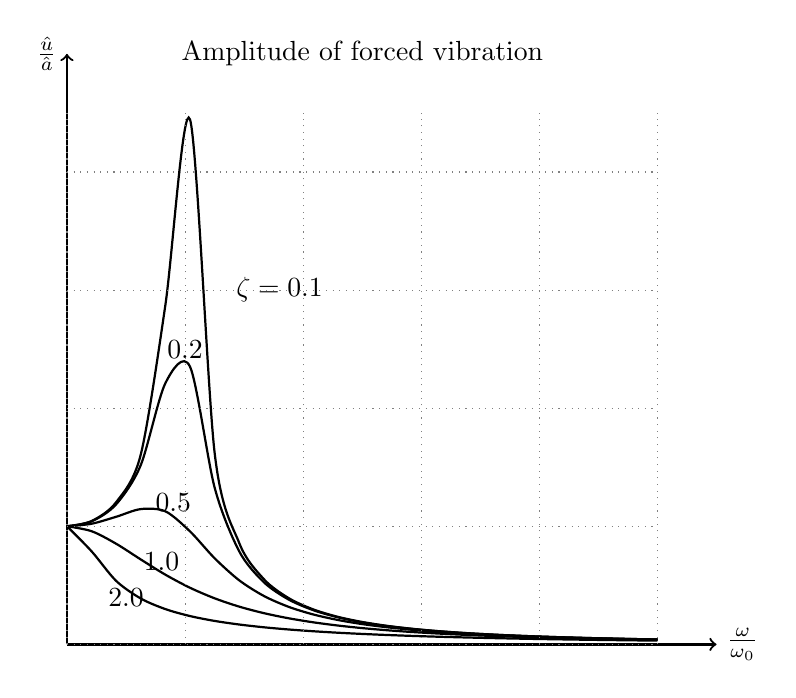
\begin{tikzpicture}[scale=1.5]
    \draw[->, black, thick] (0,0) -- (5.5,0) node[right] {$\frac{\omega}{\omega_0}$};
    \draw[->, black, thick] (0,0) -- (0, 5) node[left] {$\frac{\hat{u}}{\hat{a}}$};
    

    \draw[domain = 0:5, color = black, thick] plot[smooth] (\x,{1 / sqrt((1-\x^2)^2 + (2*0.1*\x)^2)}) node at (1.8, 3) {$\zeta = 0.1$};
    \draw[domain = 0:5, color = black, thick] plot[smooth] (\x, {1 / sqrt((1-\x^2)^2 + (2*0.2*\x)^2)}) node at (1, 2.5) {$0.2$};
    \draw[domain = 0:5, color = black, thick] plot[smooth] (\x, {1 / sqrt((1-\x^2)^2 + (2*0.5*\x)^2)}) node at (0.9, 1.2) {$0.5$};
    \draw[domain = 0:5, color = black, thick] plot[smooth] (\x, {1 / sqrt((1-\x^2)^2 + (2*1.0*\x)^2)}) node at (0.8, 0.7) {$1.0$};
    \draw[domain = 0:5, color = black, thick] plot[smooth] (\x, {1 / sqrt((1-\x^2)^2 + (2*2.0*\x)^2)}) node at (0.5, 0.4) {$2.0$};
    
    %Grid
    \draw[gray, dotted] grid (5,4.5);
    
    \node at (2.5, 5) {Amplitude of forced vibration};
\end{tikzpicture}

    \begin{minipage}[t]{.49\linewidth}
        geg.:
        \begin{tasks} (1)
            \task[] $m = \SI{3}{\kilo\gram}$
            \task[] $\omega_{gemessen} = \SI{10}{\radian\per\second}$
            \task[] $0 < \zeta < 1$
            \task[] $\zeta_{gemessen} = 0.1$
        \end{tasks}
        \end{minipage}
        \begin{minipage}[t]{.49\linewidth}
        ges.:
        \begin{tasks}
            \task$k$
        \end{tasks}
    \end{minipage}\\
    \vspace{1cm}

\underline{Zusatzfrage:} Je nach Messprinzip, wird entweder die ungedämpfte
    Eigenfrequenz, die gedämpfte Eigenfrequenz oder die maximale Anwortamplitude
    hervorrufende Anregungsfrequenz direkt erfasst. Wie groß ist für $\zeta = 0.1$ der
    Fehler bei der Schätzung von $k$, wenn man diese Frequenzen gleichsetzt?

    \begin{solution}
        \begin{alignat*}{2}
            &\text{ungedämpfte Eigenkreisfrequenz  } \omega_0 = \sqrt{\frac{k}{m}} \\
            &k_{ungedaempft} = m \cdot \omega_{gemessen}^2 &&= \SI{300.000}{\newton \per \meter} \\
            &\text{gedaempfte Eigenfrequenz  } \omega_1 = \omega_0 \sqrt{1-\zeta^2} \\
            &\omega_{gedaempft} = \frac{\omega_{gemessen}}{\sqrt{1-\zeta_{gemessen}^2}} &&= 10.05\\
            &k_{gedaempft} = m \cdot \omega_{gedaempft}^2 &&= \SI{303.030}{\newton \per \meter}\\
            &\Delta = 100 \cdot \frac{|k_{gedaempft} - k_{ungedaempft}|}{k_{ungedaempft}} &&= 1.01 \%\\
            &\text{maximale Antwortamplitude bei der Anregungsfrequenz  } \omega_{MA} = \omega_0 \sqrt{1-2 \zeta^2} \\
            &\omega_{MA} = \frac{\omega_{gemessen}}{\sqrt{1-2\zeta_{gemessen}^2}} &&= 10.102\\
            &k_{MA} = m \cdot \omega_{MA}^2 &&= \SI{306.122}{\newton \per \meter}\\
            &\Delta = 100 \cdot \frac{|k_{MA} - k_{ungedaempft}|}{k_{ungedaempft}} &&= 2.04 \% \\ 
        \end{alignat*}
    \end{solution}


		   \subsection{Frequenzanalyse}
		   \question{Berechnen Sie die Antwort des gedämpften Einmassenschwingers aus Aufgabe~\ref{question_harmonic_oscillator} auf das Sägezahnsignal $(T = \SI{1}{\second}, u_{\max} = - u_{\min} = \SI{0.1}{\meter})$,
welches durch eine Fourierreihe bis $N = 2$ approximiert werden soll. Als
Anfangsbedingungen gelten: $u(-T/2) = \SI{0}{\meter}, \dot{u}(-T/2) = \SI{0}{\meter\per\second}
$.}

\begin{tabular}{cc}
 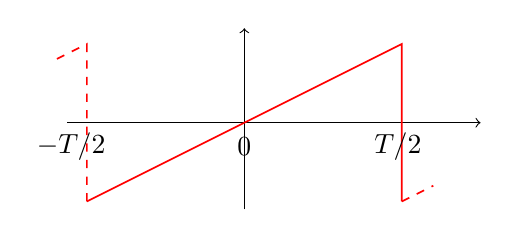
\begin{tikzpicture}[baseline=0mm] 
\draw[->] (-2.25, 0) -- (3, 0);
\draw[->] ( 0,-1.1) -- (0, 1.2);
\draw[semithick,red] (-2,-1) -- ( 2, 1) -- (2,-1);
\draw[semithick,red, dashed] (-2,-1) -- (-2, 1) -- (-2.4, 0.8);
\draw[semithick,red, dashed] ( 2,-1) -- ( 2.4,-0.8);
\draw (-2.2,-0.3) node {$-T/2$};
\draw ( 0,-0.3) node {$0$};
\draw ( 1.95,-0.3) node {$T/2$};
\end{tikzpicture}
 
 &
     $\begin{array}{l}
     a(t) = \frac{2a_{\max}}{T}t -nT\\[2mm]
     nT - \frac{T}{2} < t \leq nT + \frac{T}{2}
     \end{array}$
\end{tabular}   
     

\begin{solution}
\begin{minipage}[c]{.49\linewidth}
 \begin{align*}
     a(t) &= ct \\
     c &= \frac{2a_{\max}}{T} \\
     \tilde{w}_k &= \frac{2\pi k}{T}
 \end{align*}
\end{minipage}

\vspace{1em}

\begin{align*}
    \intertext{\flushleft Benötigte Integrale:}
    \int x \sin(ax) \dd{x} &= \frac{\sin(ax) - x \cos(ax)}{a} \\
    \int x \cos(ax) \dd{x} &= \frac{\cos(ax) + x \sin(ax)}{a}
\end{align*}

a) Darstellung der Anregung als Fourierreihe ($N=2$)

\begin{align*}
    A_0 &=  \frac{2}{T} \int\limits_{-\frac{T}{2}}^{\frac{T}{2}} a(t)\dd{t} = \frac{2}{T} \int\limits_{-\frac{T}{2}}^{\frac{T}{2}} ct \dd{t} = \frac{2}{T} \,\Big|\, \frac{c}{2}t^2\,\Big|_{t = -\frac{T}{2}}^{\frac{T}{2}} = \uuline{0}\\
    A_k &= \frac{2}{T} \int\limits_{-\frac{T}{2}}^{\frac{T}{2}} a(t) \cos(\overbrace{\frac{2\pi k}{T}}^{\tilde{w}_k}t)\dd{t} = \frac{2}{T} \int\limits_{-\frac{T}{2}}^{\frac{T}{2}} ct \cos(\tilde{w}_k t) \dd{t} \\
    &= \frac{2}{T} \,\Big|\,\frac{c}{\tilde{w}_k} (\cos(\tilde{w}_k t) + t \sin(\tilde{w}_k t))\,\Big|_{t = -\frac{T}{2}}^{\frac{T}{2}} = \uuline{0}
\end{align*}


\begin{minipage}[t]{.49\linewidth}

      $\cos(\tilde{w}_k t)$\\

    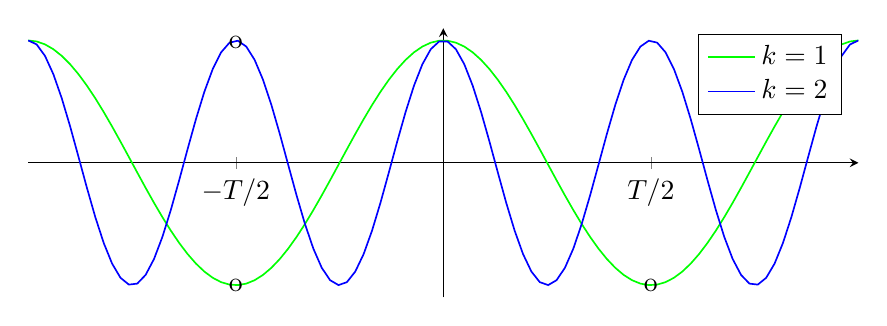
\begin{tikzpicture}
    \begin{axis}[
        width = \linewidth,
        height = 5cm,
        axis x line=center,
        axis y line=middle,
        samples=100,
        ymin=-1.1, ymax=1.1,
        xmin=-pi, xmax=pi,
        ytick=\empty,
        xtick={-pi/2,pi/2},
        xticklabels={$-T/2$,$T/2$}
        ]
        \addplot [semithick, green, domain=-pi:pi] {cos(2*deg(x))};
        \addlegendentry{$k=1$};
        \addplot [semithick, blue, domain=-pi:pi] {cos(4*deg(x))};
        \addlegendentry{$k=2$};
        \draw (axis cs: -1.57,0.98) node {o};
        \draw (axis cs: -1.57,-1) node {o};
        \draw (axis cs:  1.57,-1) node {o};
    \end{axis}
\end{tikzpicture}

\end{minipage}
\begin{minipage}[t]{.49\linewidth}

    $\sin(\tilde{w}_k t)$\\

    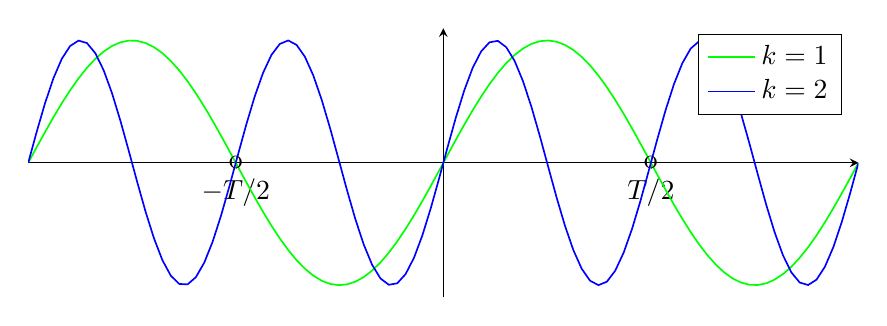
\begin{tikzpicture}
    \begin{axis}[
        width = \linewidth,
        height = 5cm,
        axis x line=center,
        axis y line=middle,
        samples=100,
        ymin=-1.1, ymax=1.1,
        xmin=-pi, xmax=pi,
        ytick = \empty,
        xtick={-pi/2,pi/2},
        xticklabels={$-T/2$,$T/2$}
        %legend style={draw=none}
        ]
        \addplot [semithick, green, domain=-pi:pi] {sin(2*deg(x))};
        \addlegendentry{$k=1$};
        \addplot [semithick, blue, domain=-pi:pi] {sin(4*deg(x))};
        \addlegendentry{$k=2$};
        \draw (axis cs: -1.57,0) node {o};
        \draw (axis cs:  1.57,0) node {o};
    \end{axis}
\end{tikzpicture}

\end{minipage}
\vspace{1em}

\begin{align*}
     B_k &= \frac{2}{T} \int\limits_{-\frac{2}{T}}^{\frac{2}{T}} ct \sin(\tilde{w}_k t) \dd{t} = \frac{2}{T}\,\Big|\, \frac{c}{\tilde{w}_k}(\sin(\tilde{w}_k t)-t\cos(\tilde{w}_k t))\,\Big|_{t={-\frac{2}{T}}}^{t=\frac{2}{t}} \\
     &= \frac{-2c}{\tilde{w}_k} \cos(\tilde{w}_k\frac{T}{2}) =
     \left\{
     \begin{array}{lll}
     \cfrac{2c}{\tilde{w}_k} & &k = 1,3,5,\dots\\[1em]
     -\cfrac{2c}{\tilde{w}_k} & &k = 2,4,6,\dots
     \end{array}\right.
\end{align*}

\begin{align*}
     \begin{array}{lcl}
        a = \overbrace{B_1\sin(\tilde{w}_1 t)}^{a_1(t)} + \overbrace{B_1\sin(\tilde{w}_2 t)}^{a_2(t)} & \rightsquigarrow & u_p(t) = u_{p1}(t) + u_{p2}(t) \\[1em]
        B_1 = \cfrac{4a_{\max}\cancel{T}}{2\pi\cancel{T}} \qquad \tilde{w}_1 = \cfrac{2\pi}{T} && u_{p1}^{(t)} = u_{C1} \cos(\tilde{w}_1 t) + u_{S1} \sin(\tilde{w}_1 t) \\[1em]
        B_2 = \cfrac{4a_{\max}}{4\pi} \qquad \tilde{w}_2 = \cfrac{4\pi}{T}&& \underbrace{u_{p2}^{(t)} = u_{C2} \cos(\tilde{w}_2 t) + u_{S2} \sin(\tilde{w}_2 t)} \\
        &&\text{Partikuläre Lösung - siehe Übung}\\
        &&\text{harmonisch erregter Einmassenschwinger}
    \end{array}
\end{align*}\\[2em]

b) Anpassung der Gesamtlösung an die Anfangsbedingungen
    
    Die Gesamtlösung setzt sich additiv aus der Lösung der homogenen Gleichung und der bereits bestimmten Partikulärlösung zusammen
    \begin{align*}
        u(t) &= C_1\cos(\omega_1 t)e^{-\delta t} + C_2 \sin(\omega_1 t)e^{-\delta t} + u_p(t),\\
        \dot{u}(t) &= -C_1 \exp(-\delta t) \cdot (\omega_1 \sin(\omega_1 t) + \delta \cos(\omega_1 t)) \\ 
        &+ C_2 \exp(-\delta t) \cdot (\cos(\omega_1 t) + \sin(\omega_1 t)) + \dot{u_p}(t).\\
    \end{align*}

    Mit den Anfangsbedingungen

    \begin{align*}
        u(t_0) &= u_0 \\
        \dot{u}(t_0) &= \dot{u}_0
    \end{align*}

    liegen zwei Gleichungen mit zwei Unbekannten vor

    \begin{align*}
        \begin{bmatrix}
            A_{11} & A_{12}\\
            A_{21} & A_{22}
        \end{bmatrix}
        \begin{bmatrix}
            C_1 \\
            C_2
        \end{bmatrix}
        &=
        \begin{bmatrix}
        b_1 \\
        b_2
        \end{bmatrix} 
        \end{align*}
        mit den Koeffizienten $A_{ij}$ und der rechten Seite $b_i$
        \begin{align*}
            A_{11}&= -\omega_1 \sin(\omega_1 t) \exp(-\delta t),\\
            A_{12}&= - \delta \cos(\omega_1 t) \exp(-\delta t),\\
            A_{21}&= \cos(\omega_1 t) \exp(-\delta t),\\
            A_{22}&= \sin(\omega_1 t) \exp(-\delta t),\\
            b_{1}&= -u_{C_1} \tilde{\omega_1} \sin(\tilde{\omega_1}t) + u_{S_1} \tilde{\omega_1} \cos(\tilde{\omega_1}t),\\
            b_{2}&= -u_{C_2} \tilde{\omega_2} \sin(\tilde{\omega_2}t) + u_{S_2} \tilde{\omega_2} \cos(\tilde{\omega_2}t).
    \end{align*}
    Es ergeben sich die folgenden Zahlenwerte
            \begin{align*}
            t_0 &= \SI{0.5}{\second}\\
            T_a &= \SI{9}{\second} \\
            k &=  \SI{10}{\newton \per \second} \\
            c &= \SI{1}{\newton \second \per \meter} \\
            a_{C_1} &= 0 \\
            a_{S_1} &= 1 \\
            \omega &= \frac{2 \pi}{T_a} &= 0.698 \\
            \omega_0 &= \sqrt{\frac{k}{m}} &= 1.826\\
            \zeta &= \frac{c}{2 \sqrt{km}} &= 0.091\\
            \eta &= \frac{\omega}{\omega_0} &= 0.382\\
            V &= \frac{1.0}{\sqrt{{(1-\eta^2)}^2 - {(2 \zeta \eta)}^2}} &= 1.608\\
            u_{C_1}  &= V^2 ((1-\eta^2) a_{c_1} - 2 \zeta \eta a_{s_1}) &= -0.095 \\ 
            u_{S_1} &= V^2 ((1-\eta^2) a_{s_1} - 2 \zeta \eta a_{c_1}) &= 1.163 \\  
            u_{p_1}(t) &= u_{C_1} \cos(\omega t) + u_{S_1} \sin(\omega t) &= -0.095 \cos(0.698 t) + 1.163 \sin(0.698 t)\\
            a_{C_2} &= \SI{0.2}{\meter} \\
            a_{S_2} &= \SI{0.0}{\meter} \\
            u_{C_2} &= V^2 ((1-\eta^2) a_{C_2} - 2 \zeta \eta a_{S_2}) &= 0.442\\
            u_{S_2} &= V^2 ((1-\eta^2) a_{s_1} - 2 \zeta \eta a_{c_1}) &= -0.036\\
            u_{p_2}(t) &= u_{C_2} \cos(2\omega t) + u_{S_2} \sin(2\omega t) &= 0.442 \cos(1.396t) -0.036 \sin(1.396 t) \\
            \omega_1 &= \omega_0 \cdot \sqrt{1 - \zeta^2} &= 1.818\\
            \intertext{aus Aufgabe\ref{question_harmonic_oscillator}} \\
            \delta &= 1.01 \% &= 0.0101\\
        \end{align*}
            Aufgelöst nach den gesuchten Koeffizienten lautet dieses Gleichungssystem
    \begin{align*}
        &\begin{bmatrix}
            C_1 \\
            C_2
        \end{bmatrix}
        = \cfrac{1}{A_{11}A_{22}-A_{12}A_{21}}
        \begin{bmatrix}
            A_{22} & -A_{12}\\
            -A_{21} & A_{11}
        \end{bmatrix}
        \begin{bmatrix}
            b_1 \\
            b_2
        \end{bmatrix}
        \end{align*}
            $A_{11} = -1.427$,
            $A_{12} = -0.006$,
            $A_{21} = 0.611$,
            $A_{22} = 0.785$,
            $b_1 = 0.786$,
            $b_2 = -0.435$.
    \begin{align*}
        \begin{bmatrix}
            C_1 \\
            C_2
        \end{bmatrix}
        = \cfrac{1}{-1.427 \cdot 0.785 + 0.006 \cdot 0.611}
        \begin{bmatrix}
            0.785 & 0.006 \\
            0.611 & -1.427
        \end{bmatrix}
        \begin{bmatrix}
            -0.550 \\
            0.438
        \end{bmatrix}          
    \end{align*}
        Als Gesamtlösung folgt
    \begin{align*}
        u(t) &= -0.550 \cos{1.818 t} \cdot \exp(-0.0101 t) + 0.438 \sin(1.818 t) \exp(-0.0101 t) + u_p(t) \\
        u_p(t) &= u_{p_1}(t) + u_{p_2}(t) \\
        & = -0.095 \cos(0.698 t) + 1.163 \sin(0.698 t) + 0.442 \cos(1.396t) -0.036 \sin(1.396 t)
    \end{align*}
\end{solution}

		   \subsection{Mechanisches Bodenverhalten}
		   \begin{questions}
    \question{Dämpfungskapazität des äquivalent-linearen Modells}
    \vspace{1em}

        \begin{minipage}[t]{.49\linewidth}
        geg.:
            \begin{tasks} (1)
                \task[] $F_D = 2\, \zeta\, \eta\, k\, \hat u\, \sin(a\, t)$
                \task[] $\dot{u} = \omega\,\hat u\, \sin(a\,t)$
            \end{tasks}
        \end{minipage}
        \begin{minipage}[t]{.49\linewidth}
        ges.:
            \begin{tasks}
                \task[] dissipierte Energie $\Delta W$ pro Zyklus
                \task[] maximal in Feder gespeicherte Energie $W$
                \task[] Dämpfungskapazität $\Psi$
            \end{tasks}
        \end{minipage}
    \vspace{1cm}

    \begin{solution}
        \begin{align*}
            W_D &= \int_{0}^{T} -F_D \dot{u} \dd{t}\\
            \intertext{für $\phi = [0, 2\pi]$} \\
            W_D &= \int_{0}^{2 \pi} F_D \dot{u} \dd{t} &&= 2 \pi \hat{u}^2 \eta k \zeta\\
            \intertext{Maximale, in Feder gespeicherte Energie:} \\
            W_{F_{\max}} &= 0.5 k \hat{u}^2 \\
            \intertext{Dämpfungskapazität:} \\
            \psi &= \frac{W_D}{W_{F_{\max}}} &&= 4.0 \pi \eta \zeta \\
        \end{align*}
    \end{solution}


\question{Schubmodul und Dämpfung bei mittleren Dehnungen}
    \vspace{1em}

    \begin{minipage}[t]{.49\linewidth}
    geg.:
        \begin{tasks} (1)
            \task[] $\hat\gamma = 0,5\%$
            \task[] $I_p = 10 \%$
        \end{tasks}
    \end{minipage}
    \begin{minipage}[t]{.49\linewidth}
    ges.:
        \begin{tasks}
            \task[] $\cfrac{G}{G_{\max}}$
            \task[] $D$
        \end{tasks}
    \end{minipage}

    \begin{center}\fbox{\underline{Hinweis:} siehe Kap. 4.2.4 Grundbau-Taschenbuch}\end{center}

    \begin{solution}
        \begin{align*}
            \frac{G}{G_{max}} 
            & = \frac{1.03}{1+\frac{19 \gamma^{0.8}}{1+ \frac{I_P}{15.0}^{1.3}}} \leq 1  
            & & \gamma \leq 1 \% \\
            D 
            & = 2 + \frac{24.5 - 0.2 I_P}{1 + \frac{1}{7.4 - 0.1 I_P} \gamma^{0.8}} \leq 1 
            & & \gamma \leq 1 \%, I_P \leq 50 \% 
            \end{align*}
            mit den gegebenen Werten
            \begin{align*}
            \frac{G}{G_{max}} &= 0.809,\\
            D &= 26.432.
        \end{align*}
    \end{solution}
\vspace{1cm}

\question{Schubmodul bei sehr kleinen Dehnungen}
\vspace{1em}

     \begin{minipage}[t]{.49\linewidth}
        geg.:
        \begin{tasks} (2)
            \task[] $n = 0.5$
            \task[] $e = 2.0$
            \task[] $I_p = 0.6$
            \task[] $P_a = 100 kPa$
            \task[] $\bar \sigma' = 1 MPa$
            \task[] $OCR = 5$
            \task[] $S = 625$
        \end{tasks}
    \end{minipage}
    \begin{minipage}[t]{.49\linewidth}
    ges.:
        \begin{tasks}
            \task[] $- G_{\max|NC}$
            \task[] $- G_{\max|OC}$
        \end{tasks}
    \end{minipage}
    \begin{center}\fbox{\underline{Hinweis:} siehe Kap. 4.2.2 Grundbau-Taschenbuch}\end{center}

    \begin{solution}
        \begin{align*}
            F_e &= \frac{1}{0.3 + 0.7 e^2} &&= 0.323\\
            G_{\max | NC} &= S\ F_e\ P_a\ (\frac{\bar \sigma'}{P_a})^n &&= \SI{63.76}{\mega \pascal} \\
            k &= \frac{I_P}{(1+ 3 I_P^2)^{0.5}} &&= 0.416 \\
            G_{\max | OC} &= G_{\max | NC}\cdot OCR^k &&= \SI{124.54}{\mega \pascal}\\
        \end{align*}
    \end{solution}

  \question{Masing-Hypothese, geometrische Konstruktion}
\vspace{1em}
    \begin{tasks}
        \task[] Zeichnen sie die Skelettkurve (punktweise Berechnung).
        \task[] Konstruieren sie für $\cfrac{\hat \gamma}{\gamma_r}=2$ (Faktor 2) die Hysterese-Äste.
    \end{tasks}

    \begin{align*}
        \cfrac{\tau}{\tau_m} = \cfrac{\cfrac{\gamma}{\gamma_r}}{1+|\cfrac{\gamma}{\gamma_r}|}
    \end{align*}

    %\includegraphics[width=0.99\textwidth]{fig_gnuplottex/graph_template.png}
    graph\_template


    \begin{solution}
        %\includegraphics[width=0.5\textwidth]{fig_gnuplottex/skeleton_curve.png}
        skeleton\_curve

    \end{solution}
    
\end{questions}

		
		\newpage
		\section{Wellenausbreitung im Untergrund}
		   \subsection{Dehnstabsmodell (1D)}
		   \question{Ein Pfeil wird auf eine Zielscheibe geschossen und bleibt stecken. Warum fliegt das Endstück Rückwärts weg?}

Fig TODO Dominik

\begin{tasks}(1)
    \task[$\bullet$] Skizzieren Sie den Kraft- und Geschwindigkeitsverlauf im Pfeil (Dehnstab)
    \task[$\bullet$] Vergleichen sie Ihr Ergebnis mit einem Einmassenschwinger, der gegen die Wand fliegt.
\end{tasks}

\begin{solution}
\flushleft HIER BITTE NOCH LÖSUNG NACHTRAGEN (Dominik Kern)
\end{solution}

\question{Ein halbunendlicher Stab wird am Rand harmonisch angeregt.

\vspace{1cm}

\begin{figure}[h]
    \centering
    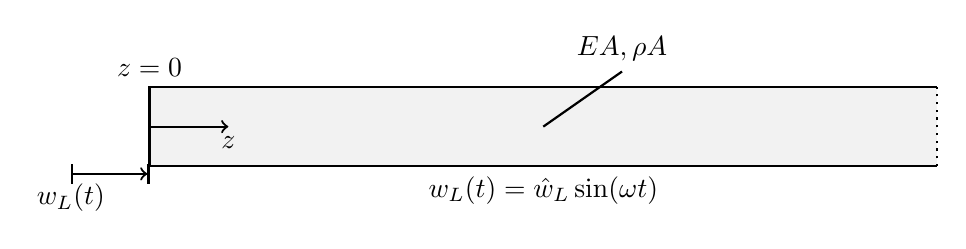
\begin{tikzpicture}
        \draw[thick, fill=gray!10] (10,0) -- node [midway, below] {$w_L (t) = \hat{w}_L \sin(\omega t)$} (0,0) -- (0,1) node[above] {$z=0$} -- (10,1) ;
        \draw[thick, dotted] (10,0) -- (10,1);
        %\draw[thick, ->] (10,0.5) -- (11,0.5);
        \draw[thick, ->] (0,0.5) -- (1,0.5) node[left, below] {$z$} ;
        \draw[thick, |->|] (-1,-0.1) node[below] {$w_L (t)$} -- (0,-0.10);
        \draw[thick] (5,0.5) -- (6,1.2) node[above] {$EA,\rho A$};
    \end{tikzpicture}
\end{figure}


Am Anfang $(t=0)$ ist er undeformiert und in Ruhe. Lösen Sie diese Aufgabe, indem Sie auf dem gedanklich über den Rand verlängerten Stab eine nach rechts laufende Welle annehmen, welche genau die vorgegebene Randbewegung erzeugt. Interpretieren Sie die Parameter dieses Verlaufs physikalisch, Stichwort ``Wellenlänge".
}

\begin{solution}
    
    \begin{align*}
        \intertext{Aus dem D'alembertschen Wellenansatz mit $t = 0$}
        &w_0(z) = \Psi(z) + \Phi(z)
        &\dot{w_0}(z) = c\Psi^{'}(z)-c\Psi^{'}(z)
        \intertext{folgt:}
        &\Psi(z) = C_1 \cos(\kappa z) + C_2 \sin(\kappa z)
        &\Phi(z) = R_1 \cos(\kappa z) + R_2 \sin(\kappa z)
    \end{align*}
\end{solution}

\question{Berechnen Sie das Reflektionsverhalten diskreter Elemente am Rand: Feder, Dämpfer und Masse.

\begin{tikzpicture}[scale=0.6]
\fill[black!25!white] (4,-1.5) rectangle +(1.5, 3); 
\fill[black!10!white] (5.5,-0.5) rectangle +(5.5, 1);  
\draw (0, 0) pic [scale=0.6] {DKbase};
\draw (0, 1) pic [scale=0.6, thick] {DKspring=4};
\draw (0,-1) pic [scale=0.6, thick] {DKdashpot=4};  
\draw[thick] (4,-1.5) rectangle +(1.5, 3); 
\draw[thick] (5.5, -0.5) -- (11, -0.5);
\draw[thick] (5.5,  0.5) -- (11,  0.5);
\draw (2.0, 0.1) node {$k$};
\draw (2.0,-1.9) node {$c$};
\draw (4.75, 0) node {$m$};
\draw (8, 0) node {$E$,$A$,$\rho$};
\end{tikzpicture}


Nehmen Sie dazu eine einfallende nach links laufende Welle $w_{ein}(z,t) = C_1 \cos(kz+\omega t)$ an und 
berechnen Sie die reflektierende Welle $w_{ref}(z,t)=R_1\cos(kz-\omega t) + R_2 \sin(kz-\omega t)$. \\
\qquad

\fbox{Hinweis ($z=0$):}
\begin{tasks} (3)
    \task[] $kw = EAw'$
    \task[] $c\dot w = (EA)w'$
    \task[] $m\ddot w = (EA)w'$
    \task[] Feder-RB
    \task[] Dämpfer-RB
    \task[] Masse-RB
\end{tasks}

\fbox{
    \begin{minipage}[t]{\textwidth}
        Hinweis: Der Punkt steht für die Ableitung nach der Zeit $t$, \\der Apostroph für die Ableitung nach der räumlichen Koordinate $z$.
    \end{minipage}}
}    

\begin{solution}
        Ableitungen der Funktion $w$:
        \begin{align*}
            \dot{w} &= -C_1 \omega \sin(\kappa z + \omega t) + C_2 \omega \cos(\kappa z + \omega t) \\
                     &+ R_1 \omega \sin(\kappa z - \omega t) - R_2 \omega \cos(\kappa z - \omega t) \\
            \ddot{w} &= - C_1 \omega^2 \cos(\kappa z + \omega t) - C_2 \omega^2 \sin(\kappa z + \omega t) \\
                     &-R_1 \omega^2 \cos(\kappa z - \omega t) - R_2 \omega^2 \sin(\kappa z - \omega t) \\
            w^{'} &= -C_1 \kappa \sin(\kappa z + \omega t) + C_2 \kappa \cos(\kappa z + \omega t) \\
                   &-R_1 \kappa \sin(\kappa z - \omega t) + R_2 \kappa \cos(\kappa z - \omega t)
        \end{align*}

        Schrittweise Berechnung der Reflektion: \\
        1. Anfangsbedingung: $z=0$ \\
        2. Ausklammern der Sinus- und Cosinus-Ausdrücke (am besten in Matrixform)\\
        3. Aus den erhaltenen Koeffizienten der Sinus- und Cosinusfunktionen kann nun nach $R_1$ und $R_2$ umgestellt werden.
            Dabei ergibt sich $R_1$ aus den Koeffizienten des Kosinus und $R_2$ aus den Sinuskoeffizienten.\\

        Feder:
        \begin{align*}
            0 &= kw - EA  w^{'}\\
            R_1 &= \frac{C_1 {(EA)}^2 \kappa^2 - C_1 k^2 + 2C_2 (EA) k \kappa}{{(EA)}^2 \kappa^2 + k^2}\\
            R_2 &= \frac{2C_1 (EA) k \kappa - C_2 {(EA)}^2 \kappa^2 + C_2 k^2}{{(EA)}^2 \kappa^2 + k^2}
        \end{align*}
        Dämpfer:
        \begin{align*}
            0 &= c \dot{w} - EA  w^{'}\\
            R_1 &= \frac{C_1 (EA) \kappa - C_1 c w}{(EA) \kappa + cw}\\
            R_2 &= \frac{-C_2 (EA) \kappa + C_2 cw}{(EA) \kappa + cw}
        \end{align*}
        Masse:
        \begin{align*}
            0 &= m \ddot{w} - (EA) w^{'}\\
            R_1 &= \frac{C_1 {(EA)}^2 \kappa^2 - C_1 m^2 \omega^4 - 2C_2 (EA) \kappa m \omega^2}{{(EA)}^2 \kappa + m^2 \omega^4}\\
            R_2 &= \frac{-2C_1 (EA) \kappa m \omega^2 - C_2 {(EA)}^2 \kappa^2 + C_2 m^2 \omega^4}{{(EA)}^2 \kappa + m^2 \omega^4}
    \end{align*}
\end{solution}

\question{Resonant Column}
TODO Dominik Kern (siehe V09aufgaben.pdf) stehende Welle

\vspace{1cm}

\begin{tikzpicture}
\draw[thick, fill=black!10!white] (-0.2, 0) rectangle (0.2, 3.0);
\draw[thick, fill=black!20!white] (-0.5, 3) rectangle (0.5, 3.5);
\draw(1, 3.2) node[right] {$J$};
\draw(1, 1.5) node[right] {$G,I,\rho$};
\draw (0, 0) pic [rotate=90, scale=0.5] {DKbase};
\draw[<->, thin] (-0.4, 0) -- node[left] {$l$} (-0.4, 3);
\draw[thin] (0.1, 1.0) -- (1.0, 1.5);
\draw[thin] (0.4, 3.3) -- (1.1, 3.2);
\end{tikzpicture}


		   \subsection{Elastodynamik (3D)}
		   TODO Elastodynamikaufgaben

		
		\newpage
		\section{Praktische Anwendung}
		   \subsection{Kennwertermittlung}
		   TODO Dominik Kern

\bigskip

E-Modul aus Zugversuch, Eigenfrequenz, und Wellengeschwindigkeit 
und oder Schubmodul aus Scher-, Torsionsversuch und Resonant Column (siehe V09aufgaben.pdf)
(reale Daten, z.B. YS)




		   \subsection{Konstruktionskriterien}
		   Erdbebenersatzkraft anhand des Bemessungsspektrums

\smallskip

TODO Aufgabe V09aufgabe.pdf (handschriftlich)


\question{Erdbebenbemessungspektren}

Ermitteln Sie für ein zweigeschossiges Gastronomiegebäude in Holzbauweise die Gesamterdbebenkraft in horizontaler Richtung
aus dem Bemessungsspektrum.

\begin{minipage}[t]{\linewidth}
    geg:
    \begin{tasks} (2)
        \task[] Erdbebenzone 3
        \task[] $a_{gR} = \SI{0.8}{\metre\per\second^2}$
        \task[] Bedeutungskategorie \romannum{3}
        \task[] $\gamma = 1.2$
        \task[] Untergrundklasse B-R
        \task[]
        \task[] Duktilitätsklasse 1
        \task[] $q = 1.5$
        \task[] Masse: $m =\SI{80}{\tonne}$
        \task[] Gesamthöhe: $h = 6m$
    \end{tasks}
\end{minipage}

Formeln und Parameter aus [Schmidt, Buchmaier, Vogt-Beyer: Grundlagen der Geotechnik, 5. Auflage, S.725f.]

\begin{align*}
    &0 < T \leqq T_B: &&S_d(T) = a_{gR} \gamma_l S [1 + \frac{T}{T_B}(\frac{2.5}{q} -1)] \\
    &T_B \leqq T \leqq T_C: &&S_d(T) = a_{gR} \gamma_l S \frac{2.5}{q} \\
    &T_C \leqq T \leqq T_D: &&S_d(T) = a_{gR} \gamma_l S \frac{2.5}{q} \frac{T_C}{T} \\
    &T_D \leqq T \leqq 4s: &&S_d(T) = a_{gR} \gamma_l S \frac{2.5}{q} \frac{T_C T_D}{T^2} \\
\end{align*}

Anhand der Untergrundklasse B-R lassen sich folgende Parameter ablesen:
\begin{tasks} (4)
    \task[] $S = 1.25$
    \task[] $T_B in s = 0.05$
    \task[] $T_C in s = 0.25$
    \task[] $T_D in s = 2.0$
\end{tasks}

Nach \textit{DIN EN 1198-1} lässt sich die Gesamterdbebenkraft $F_b$ bestimmen.

\begin{align}
    F_b &= S_d(T_1) m \lambda
\end{align}

$T_1$ wird näherungsweise bestimmt durch:
\begin{align}
    T_1 &= C_t h^{\frac{3}{4}}
\end{align}

\begin{solution}
    
\end{solution}
	
	\end{questions}

\end{document}
